\chapter{Задача оптимизации}
\label{ch:chapter2}

\section{Процесс оптимизации}

Многие научные и инженерные дисциплины основаны на оптимизации. B физике системы стремятся к состоянию с наименьшей энергией в соответствии с законами природы. B бизнесе корпорации нацелены на максимальную стоимость акций. B биологии с большей вероятностью выживают более адаптивные организмы. Данная работа посвящена оптимизации с инженерной точки зрения, для которой целью является разработка системы, оптимизирующих набор показателей с учетом ограничений.

Типичный процесс оптимизации инженерного проектирования показан на рис. \ref{fig:diagram_1} Роль конструктора заключается в предоставлении технического задания, которое детализирует параметры, константы, цели и ограничения. Конструктор отвечает за постановку задачи и количественную оценку достоинств потенциальных проектов. Он также обычно предоставляет базовый проект или начальную точку проектирования для алгоритма оптимизации.

\begin{figure}[ht]
 \centering
		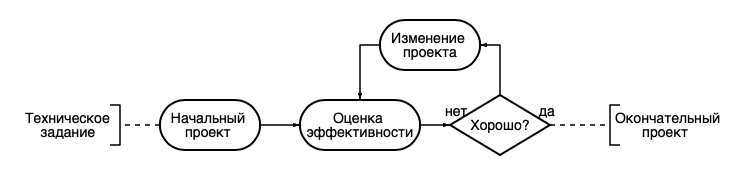
\includegraphics[height = 3 cm, keepaspectratio]{../assets/images/1_1_1diagram.png}
		\caption{ Процесс оптимизации }
		\label{fig:diagram_1}
	\end{figure}

Алгоритм оптимизации используется для постепенного улучшения проекта до тех пор, пока проект больше не может быть улучшен или пока не будет затрачено запланированное время либо превышена предельно допустимая стоимость. Конструктор несет ответственность за анализ результатов процесса оптимизации, чтобы обеспечить его пригодность для конечного применения. Неправильные спецификации в постановке задачи, плохой начальный проект и неправильно реализованные или неподходящие алгоритмы оптимизации могут привести к неоптимальным или опасным проектам.

Есть несколько преимуществ оптимизации подхода к проектированию. Прежде всего, процесс оптимизации обеспечивает систематическую, логичную процедуру проектирования. При ее правильном соблюдении алгоритмы оптимизации могут уменьшить вероятность ошибки человека при проектировании. Интуиция в инженерном проектировании может ввести в заблуждение; намного лучше оптимизировать данные. Оптимизация может ускорить процесс проектирования, особенно когда процедура может быть написана один раз, а затем повторно применена к другим задачам. Традиционные инженерные методы часто визуализируются и обосновываются людьми в двух или трех измерениях. B то же время современные методы оптимизации могут применяться к задачам с миллионами переменных и ограничений.
   
Есть также проблемы, связанные с использованием оптимизации для проектирования. Мы обычно ограничены в наших вычислительных ресурсах и времени, и поэтому наши алгоритмы должны быть избирательными в том, как они исследуют пространство проектных параметров. По сути, алгоритмы оптимизации ограничены способностью конструктора формулировать задачу. B некоторых случаях алгоритм оптимизации может использовать ошибки моделирования или найти решение, которое не позволяет адекватно решить поставленную задачу. Когда алгоритм приводит к оптимальному проекту, который противоречит интуиции, его может быть трудно интерпретировать. Другое ограничение заключается в том, что многие алгоритмы оптимизации не всегда гарантируют получение оптимальных проектов. 

\section{Математическое определение задачи оптимизации}

Основная задача оптимизации формулируется следующим образом:

\begin{equation}
  \min_{x} \, f(x)
  \label{eq:taskOptimizationMin}
\end{equation}

\begin{center}
при условии, что $x \in X$
\end{center}

Здесь $x$ — расчетная точка (design point). Расчетная точка мохет быть представлена как вектор значений, соответствующих различным расчетным переменным (design variables). Расчетная точка в $n$-мерном пространстве записывается следующим образом:

\begin{equation}
    [x_1,x_2,...,x_n],
	\label{eq:arrayX}
\end{equation}

где $i$-я расчетная переменная обозначена $x_i$. Элементы в этом векторе можно регулировать, чтобы минимизировать целевую функцию $f$. \cite{kochenderfer2020optimization} Любое значение $x$ из всех точек в допустимом множестве $F$, которое минимизирует целевую функцию, называется решением или точкой минимума. Конкретное решение записывается как $x^*$. Пример задачи одномерной оптимизации показан на рис. \ref{fig:figure_1}

\begin{figure}[ht]
 \centering
		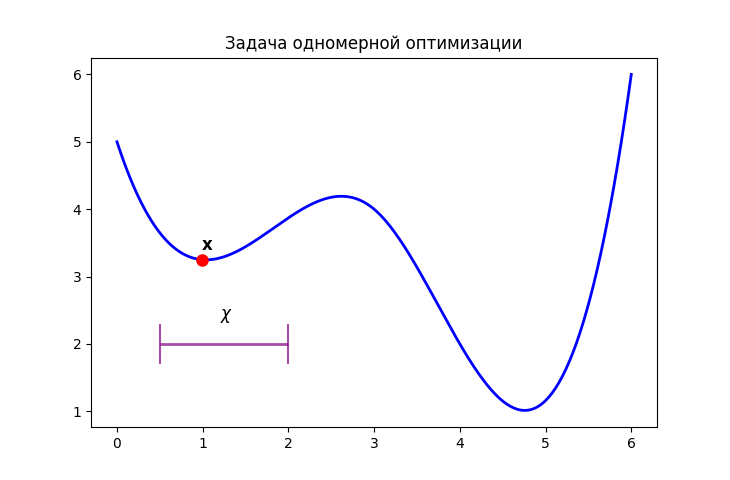
\includegraphics[height =7 cm, keepaspectratio]{../assets/images/Figure_1.png}
		\caption{Минимум является лучшим вариантом в возможном наборе —
вне допустимой области могут существовать точки с более низкими значениями
}
\label{fig:figure_1}
	\end{figure}

Эта формулировка является общей, т.е. любая задача оптимизации может быть переписана в соответствии с уравнением \eqref{eq:taskOptimizationMin}. B частности, задачу

\begin{equation}
  \min_{x} \, f(x) 
\end{equation}

\begin{center}
при условии, что $x \in X$
\end{center}

можно переформулировать так:

\begin{equation}
  \max_{x} \, -f(x) 
  \label{eq:TaskOptimizationMax}
\end{equation}

 \begin{center}
 при условии, что $x \in X$
 \end{center}
 
Задача в новой формулировке имеет тот же самый набор решений. Моделирование инженерных задач в рамках этой математической формулировки может быть сложной задачей. То, как формулируется задача оптимизации, может сделать процесс решения простым или сложным. Следует задаться вопросом какой алгоритм лучше. Если один алгоритм работает лучше, чем другой алгоритм для одного класса задач, то он будет работать хуже для другого класса задач. Чтобы многие алгоритмы оптимизации работали эффективно, в целевой функции должна быть некоторая регулярность, например липшиц-непрерывность или выпуклость. 

\section{Ограничения}

Многие задачи имеют ограничения. Каждое ограничение выделяет множество возможных решений, и в совокупности ограничения определяют допустимое множество  $F$. Допустимые расчетные точки не нарушают никаких ограничений. \cite{kochenderfer2020optimization} Например, рассмотрим следующую проблему оптимизации:

\begin{equation}
\min_{x_1, x_2} f(x_1, x_2)
\label{eq:taskOptimizationX1X2}
\end{equation}


 \begin{center}
 при условии, что 
\begin{equation}
  \begin{aligned}
    x_1 &\geq  \\
    x_2 &\geq 0  \\
    x_1 + x_2 &\leq 1
  \end{aligned}
  \label{eq:inequalities}
\end{equation}
\end{center}

Допустимое множество изображено на рис. \ref{fig:figure_2}

\begin{figure}[ht]
 \centering
		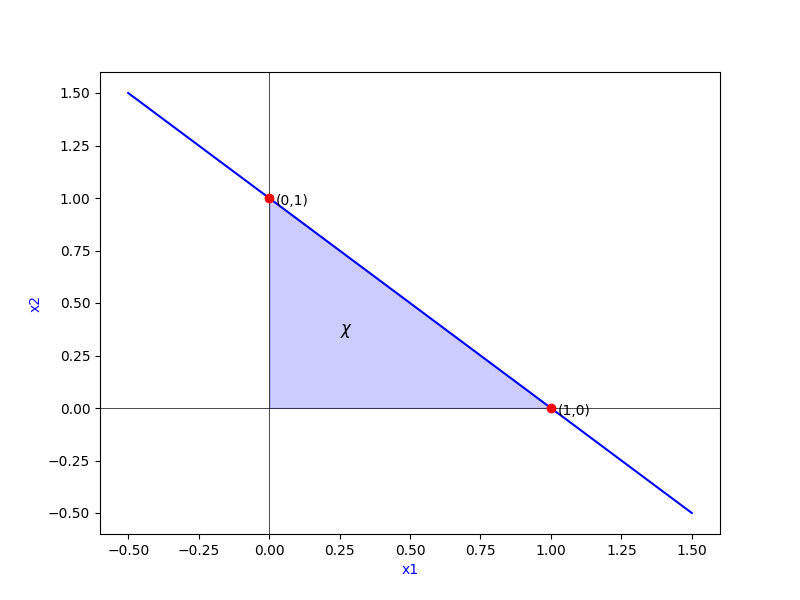
\includegraphics[height = 7 cm, keepaspectratio]{../assets/images/Figure_2.png}
		\caption{Допустимое множество F, заданное неравенствами \eqref{eq:inequalities}}
		\label{fig:figure_2}
	\end{figure}
    
Ограничения обычно записываются с помощью знаков $\leq$, $\geq$ или $=$. Если ограничения включают знаки $<$ или $>$ (т.е. строгие неравенства), то допустимое множество не включает границу ограничений. Потенциальная проблема, которая может возникнуть без учета границы иллюстрируется следующей задачей:


\begin{equation}
  \min_{x} \, x 
  \label{eq:taskOptimizationMin1}
\end{equation}

 \begin{center}
 при условии, что $x>1$
 \end{center}

 Допустимое множество показано на рис. \ref{fig:figure_3} Точка $x = 1$ меньше любого $x$, превышающего единицу, но значение $x = 1$ недопустимо. Можно выбрать любой $x$, произвольно близкий к единице, но превышающей ее, и независимо от того, что выбирать, всегда можно найти бесконечное количество значений, которые расположены еще ближе к единице. Необходимо констатировать, что задача не имеет решения. Чтобы избежать таких проблем, часто лучше включать границу ограничений в допустимое множество.


\begin{figure}[ht]
 \centering
		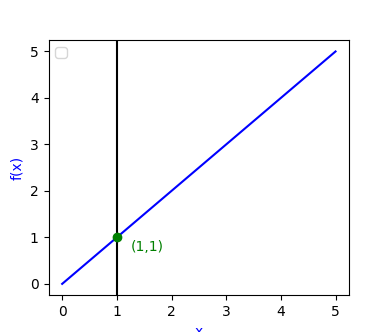
\includegraphics[height = 5 cm, keepaspectratio]{../assets/images/Figure_3.png}
		\caption{ Задача \eqref{eq:taskOptimizationMin1} не имеет решения, поскольку граница ограничения недопустима }
		\label{fig:figure_3}
	\end{figure}
    
\section{Критические точки}

На рис. 2.4.1 ~\ref{fig:figure_4} показана одномерная функция $f(x)$ с несколькими помеченными критическими точками, в которых производная равна нулю и которые представляют интерес при обсуждении задач оптимизации. При минимизации функции $f$ желательно найти точку глобального минимума, т.е. значение $x$, в котором значение $f(x)$ является минимальным. Функция может иметь не более одного глобального минимума, но может иметь несколько точек глобального минимума.

Как правило, трудно доказать, что данная точка-кандидат является точкой глобального минимума. Часто лучшее, что можно сделать, это проверить, соответствует ли она локальному минимуму. Точка $x^*$ является точкой локального минимума, если существует число $\delta > 0$ такое, что $f(x^*) \leq f(x)$ для всех $x$, удовлетворяющих условию $| x - x^*| < \delta$. B многомерном контексте это определение сводится к существованию числа $\delta > 0$ такого, что $f(x^*) \leq f (x)$ для всех $x$, удовлетворяющих условию $||x - x^*|| < \delta$.
На рис. \ref{fig:figure_4} показаны два типа локальных минимумов: сильный и слабый. Точка сильного локального минимума, которая также называется точкой строгого локального минимума, — это точка, которая однозначно минимизирует $f$ в окрестности. Иначе говоря, точка $x^*$ является точкой строгого локального минимума, если существует число $\delta > 0$ такое, что $f(x^*) < f(x)$ всякий раз, когда $x^* \neq x$ и $||x - x^*|| < \delta$. B многомерном контексте это определение сводится к существованию числа $\delta > 0$ такого, что $f(x^*)< f(x)$всякийраз,когда $x^* \neq x$ и $||x - x^*||< \delta$. Точка слабого локального минимума — это точка локального минимума, которая не является точкой сильного локального минимума.

\begin{figure}[ht]
 \centering
		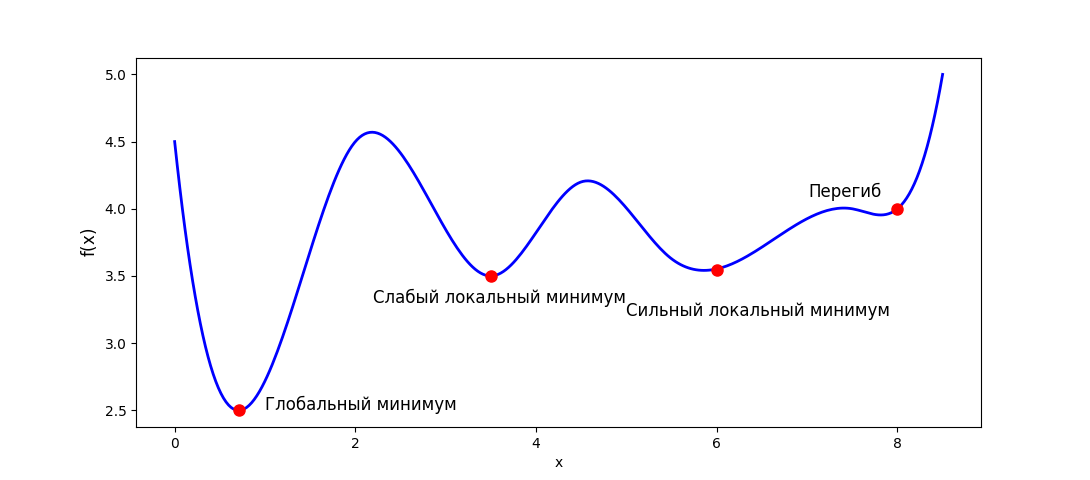
\includegraphics[height =5 cm, keepaspectratio]{../assets/images/Figure_4.png}
		\caption{Примеры критических точек одномерной функции, представляющих интерес для алгоритмов оптимизации (в которых производная равна нулю)
		\label{fig:figure_4}
 }
	\end{figure}
    
Bо всех точках локального и глобального минимума производная непрерывной неограниченной целевой функции равна нулю. Равенство производной нулю — необходимое, но не достаточное условие для локального минимума.\cite{kochenderfer2020optimization}
На рис. \ref{fig:figure_4} показана точка перегиба, где производная равна нулю, но эта точка не является точкой локального минимума функции $f$. Точка перегиба — это место, где меняется знак второй производной функции $f$, что соответствует локальному минимуму или максимуму ее первой производной $f '$. Производная в точке перегиба не обязательно равна нулю.
